\documentclass[aspectratio=169,11pt]{beamer}

\def\courseTitle{Industrial Security (Master)}
\def\courseSubtitle{Section 06 -- Threat Intelligence for OT}
\def\sectionNumber{06}
\def\sectionTitle{Threat Intelligence for OT}

% =====================================================================
% Industrial Security lecture series -- modern Beamer preamble.
%
% Each slide deck must define the following BEFORE \input{}-ing this:
%   \def\courseTitle{...}        e.g. Industrial Security (Bachelor)
%   \def\courseSubtitle{...}     e.g. Section 3 -- Network Architecture
%   \def\sectionNumber{...}      e.g. 03
%   \def\sectionTitle{...}       e.g. Industrial Network Architectures
%
% Optional:
%   \def\courseAuthor{...}       defaults to "Lecture Notes"
%   \def\courseInstitute{...}    defaults to "Department of Computer Science"
%   \def\companyLogo{...}        path to a logo image (PDF/PNG/JPG).
%
% Callout macros (use anywhere inside a frame):
%   \begin{notebox}{title}      ... \end{notebox}
%   \begin{importantbox}{title} ... \end{importantbox}
%   \begin{warningbox}{title}   ... \end{warningbox}
%   \begin{tipbox}{title}       ... \end{tipbox}
%   \begin{defbox}{title}       ... \end{defbox}
%   \begin{takeawaybox}{title}  ... \end{takeawaybox}
%   \begin{quotebox}            ... \end{quotebox}
% =====================================================================

% --- Speaker-notes mode (toggled by Makefile via -usepretex) ----------
% When notesmode=1, build a side-by-side slide+notes PDF for the
% lecturer. When unset/0, build the clean slides-only PDF.
\providecommand{\notesmode}{0}
\ifnum\notesmode=1
  \usepackage{pgfpages}
  \setbeameroption{show notes on second screen=right}
  \setbeamerfont{note page}{size=\small}
\fi

\usepackage[utf8]{inputenc}
\usepackage[T1]{fontenc}
\usepackage[english]{babel}
% Modern type pair: IBM Plex Sans for text, IBM Plex Mono for code.
% Math stays in lmodern; Plex is the dominant family on every text frame.
\usepackage{plex-sans}
\usepackage{plex-mono}
\renewcommand{\familydefault}{\sfdefault}
\usepackage[activate={true,nocompatibility},final,tracking=true,kerning=true,spacing=true,factor=1100,stretch=10,shrink=10]{microtype}
\usepackage{graphicx}
\usepackage{listings}
\usepackage{xcolor}
\usepackage{colortbl}
\usepackage{tikz}
\usepackage{booktabs}
\usepackage{array}
\usepackage{hyperref}
\usepackage{amsmath}
\usepackage{amssymb}
\usepackage{tcolorbox}
\tcbuselibrary{skins, breakable, raster}
\usepackage{fontawesome5}

% =====================================================================
% Shared TikZ styles for the Industrial Security lecture series.
% Loaded by every slide deck and exercise sheet that uses TikZ.
% =====================================================================

\usetikzlibrary{
  arrows.meta,
  shapes,
  shapes.geometric,
  shapes.symbols,
  shapes.multipart,
  positioning,
  fit,
  calc,
  backgrounds,
  decorations.pathmorphing,
  decorations.pathreplacing,
  decorations.text,
  patterns,
  matrix,
  shadows
}

% --- colour palette --------------------------------------------------
\definecolor{isOT}{HTML}{1F4E79}     % OT (deep blue)
\definecolor{isIT}{HTML}{6F2DA8}     % IT (purple)
\definecolor{isSafety}{HTML}{C00000} % safety red
\definecolor{isNet}{HTML}{2E7D32}    % network green
\definecolor{isAttack}{HTML}{B23A48} % attack red
\definecolor{isAccent}{HTML}{E08E0B} % amber
\definecolor{isMute}{HTML}{6B6B6B}   % grey
\definecolor{isLight}{HTML}{EDF2F8}  % light background
\definecolor{isPLC}{HTML}{2C5282}
\definecolor{isHMI}{HTML}{2F855A}
\definecolor{isSCADA}{HTML}{6B46C1}

% --- generic node styles --------------------------------------------
\tikzset{
  isnode/.style={
    draw, rounded corners=2pt, minimum height=8mm, minimum width=18mm,
    font=\small, align=center, thick
  },
  isbox/.style={isnode, fill=isLight},
  plc/.style={isnode, fill=isPLC!15, draw=isPLC, thick},
  hmi/.style={isnode, fill=isHMI!15, draw=isHMI, thick},
  scada/.style={isnode, fill=isSCADA!15, draw=isSCADA, thick},
  sensor/.style={isnode, fill=isNet!10, draw=isNet, minimum height=6mm, minimum width=14mm, font=\scriptsize},
  actuator/.style={isnode, fill=isAccent!15, draw=isAccent, minimum height=6mm, minimum width=14mm, font=\scriptsize},
  firewall/.style={isnode, fill=isAttack!15, draw=isAttack, thick},
  server/.style={isnode, fill=isMute!15, draw=isMute!80, thick},
  switch/.style={isnode, fill=isLight, draw=black!60, minimum height=6mm, minimum width=14mm, font=\scriptsize},
  workstation/.style={isnode, fill=white, draw=isOT, thick},
  attacker/.style={isnode, fill=isAttack!20, draw=isAttack, thick, font=\small\bfseries},
  inetnode/.style={draw, ellipse, minimum width=24mm, minimum height=10mm, font=\scriptsize, fill=isLight, thick},
  process/.style={isnode, fill=isOT!15, draw=isOT, thick, minimum width=24mm},
  zone/.style={
    draw, rounded corners=4pt, thick, dashed, inner sep=4mm
  },
  conduit/.style={-{Stealth[length=2.5mm]}, thick, isNet!80!black},
  attack/.style={-{Stealth[length=2.5mm]}, thick, isAttack, dashed},
  flow/.style={-{Stealth[length=2.5mm]}, thick, isOT!70!black},
  netline/.style={thick, black!60},
  axisline/.style={-{Stealth[length=2mm]}, thick, black!70},
  tag/.style={font=\scriptsize\itshape, fill=white, inner sep=1pt},
  level/.style={
    draw, fill=isLight, minimum width=0.85\linewidth, minimum height=8mm,
    font=\small, anchor=west
  },
  brace/.style={decorate, decoration={brace, amplitude=4pt, raise=2pt}},
  legendbox/.style={draw, rounded corners=2pt, fill=isLight, inner sep=2mm, font=\scriptsize, align=left}
}

% --- handy macros ----------------------------------------------------
% \plcicon, \hmiicon etc as simple labelled boxes; useful inline.
\newcommand{\plcicon}[1][PLC]{\tikz[baseline=-0.6ex]{\node[plc, minimum width=10mm, minimum height=5mm, font=\scriptsize, inner sep=1pt]{#1};}}
\newcommand{\hmiicon}[1][HMI]{\tikz[baseline=-0.6ex]{\node[hmi, minimum width=10mm, minimum height=5mm, font=\scriptsize, inner sep=1pt]{#1};}}
\newcommand{\fwicon}[1][FW]{\tikz[baseline=-0.6ex]{\node[firewall, minimum width=10mm, minimum height=5mm, font=\scriptsize, inner sep=1pt]{#1};}}


\graphicspath{{.}{../../../template/}}

% --- defaults --------------------------------------------------------
\providecommand{\courseAuthor}{Lecture Notes}
\providecommand{\courseInstitute}{Department of Computer Science}
\providecommand{\companyLogo}{logo}

% --- modern palette --------------------------------------------------
\definecolor{slideAccent}{HTML}{1F4E79}       % primary navy
\definecolor{slideSecondary}{HTML}{E08E0B}    % amber accent

% --- Corporate branding overrides ------------------------------------
% A user-editable `branding.tex` at the repo root can override the
% logo path, author/institute lines, and brand colours. If the file is
% missing the built-in defaults above stay in effect.
\IfFileExists{../../../branding.tex}{% =====================================================================
% Corporate / institutional branding -- single file to customise the
% look of the entire course (slides, notes, exercises, labs).
%
% HOW TO REBRAND IN UNDER A MINUTE:
%   1. Replace `branding/logo.pdf` with your own logo
%      (PDF preferred; PNG and JPG also work -- name it `logo.<ext>`).
%   2. (Optional) change the two colours below to your brand palette.
%   3. (Optional) override the author/institute lines below.
%   4. Re-run `make` at the repo root. That's it.
%
% Everything in this file has sensible defaults; you can delete a line
% to fall back to the built-in defaults, or comment it out.
%
% This file is loaded automatically by the slides, exercise, and lab
% preambles -- you never need to \input it manually.
% =====================================================================

% --- Logo --------------------------------------------------------------
% Path is resolved from each leaf-build directory; the default points at
% the shared `branding/` folder at the repo root. If you put your logo
% somewhere else, set the full or relative path here (without extension):
\renewcommand{\companyLogo}{../../../branding/logo}

% --- Author / institute (appears on the title page footer) ------------
\renewcommand{\courseAuthor}{}
\renewcommand{\courseInstitute}{}

% --- Brand colours ----------------------------------------------------
% slideAccent      = primary brand colour (title bands, accent rule)
% slideSecondary   = secondary brand colour (section badge, highlight)
% Both use HTML hex codes. Keep enough contrast against white text.
\definecolor{slideAccent}{HTML}{00205B}      % deep navy
\definecolor{slideSecondary}{HTML}{00A0DC}   % light blue accent
}{}
\definecolor{slideTitle}{HTML}{0F2A44}        % near-black navy
\definecolor{slideMuted}{HTML}{6B6B6B}
\definecolor{slideBg}{HTML}{FFFFFF}
\definecolor{slidePanel}{HTML}{F4F7FB}
\definecolor{slideRule}{HTML}{D6DEE8}

% Callout colours
\definecolor{calNote}{HTML}{1F4E79}
\definecolor{calImportant}{HTML}{B23A48}
\definecolor{calWarning}{HTML}{C77700}
\definecolor{calTip}{HTML}{2E7D32}
\definecolor{calDef}{HTML}{6B46C1}
\definecolor{calTake}{HTML}{0F2A44}

% --- beamer theme ---------------------------------------------------
\useinnertheme{rectangles}
\usefonttheme{professionalfonts}

\setbeamertemplate{navigation symbols}{}
\setbeamertemplate{itemize items}[circle]
\setbeamertemplate{enumerate items}[default]
\setbeamertemplate{section in toc}[ball numbered]
\setbeamercolor{section in toc}{fg=slideTitle}

% Colours
\setbeamercolor{normal text}{fg=slideTitle, bg=slideBg}
\setbeamercolor{title}{fg=slideAccent}
\setbeamercolor{subtitle}{fg=slideMuted}
\setbeamercolor{frametitle}{fg=slideAccent}
\setbeamercolor{structure}{fg=slideAccent}
\setbeamercolor{itemize item}{fg=slideAccent}
\setbeamercolor{itemize subitem}{fg=slideSecondary}
\setbeamercolor{block title}{fg=white, bg=slideAccent}
\setbeamercolor{block body}{fg=slideTitle, bg=slidePanel}
\setbeamercolor{alerted text}{fg=slideSecondary}

% Fonts
\setbeamerfont{title}{series=\bfseries, size=\Large}
\setbeamerfont{subtitle}{series=\mdseries, size=\normalsize}
\setbeamerfont{frametitle}{series=\bfseries, size=\large}
\setbeamerfont{block title}{series=\bfseries, size=\normalsize}
\setbeamerfont{footline}{size=\tiny}

% --- frametitle: title bar + accent underline + section badge -------
% The accent rules are wrapped in a zero-width box so they never
% contribute to the surrounding hbox width (no Overfull warnings).
\setbeamertemplate{frametitle}{%
  \nointerlineskip
  \begin{beamercolorbox}[wd=\paperwidth, ht=2.8ex, dp=1.6ex, leftskip=1.2em, rightskip=1.2em]{frametitle}%
    \usebeamerfont{frametitle}\insertframetitle%
    \hfill
    {\color{slideMuted}\small \sectionNumber}%
  \end{beamercolorbox}%
  \nointerlineskip
  \makebox[0pt][l]{\hspace*{1.2em}\textcolor{slideSecondary}{\rule{2.5em}{1pt}}\textcolor{slideAccent}{\rule{\dimexpr\paperwidth-3.7em\relax}{1pt}}}%
  \par\vskip4pt
}

% --- footer ---------------------------------------------------------
\defbeamertemplate*{footline}{is-footer}{%
  \leavevmode%
  \hbox{%
    \begin{beamercolorbox}[wd=.55\paperwidth, ht=2.4ex, dp=1ex, leftskip=1em]{author in head/foot}%
      {\color{slideMuted}\tiny \courseTitle{} \;\; $\bullet$ \;\; Section \sectionNumber{} -- \sectionTitle}%
    \end{beamercolorbox}%
    \begin{beamercolorbox}[wd=.45\paperwidth, ht=2.4ex, dp=1ex, rightskip=1em]{title in head/foot}%
      \hfill {\color{slideMuted}\tiny \insertframenumber{} / \inserttotalframenumber}%
    \end{beamercolorbox}%
  }%
  \vskip2pt
}

% --- listings -------------------------------------------------------
\definecolor{codebg}{HTML}{F4F7FB}
\definecolor{codekw}{HTML}{0F2A44}
\definecolor{codestr}{HTML}{8B3A3A}
\definecolor{codecom}{HTML}{5A7D54}

\lstset{
    backgroundcolor=\color{codebg},
    basicstyle=\ttfamily\scriptsize\color{slideTitle},
    keywordstyle=\color{codekw}\bfseries,
    stringstyle=\color{codestr},
    commentstyle=\color{codecom}\itshape,
    breaklines=true,
    frame=leftline,
    framerule=2pt,
    rulecolor=\color{slideAccent},
    numbers=left,
    numberstyle=\tiny\color{slideMuted},
    numbersep=8pt,
    showstringspaces=false,
    tabsize=2,
    captionpos=b,
    xleftmargin=0.6em
}

% --- callout boxes --------------------------------------------------
% Shared base style for all callout boxes.
% Subtle drop shadow gives the boxes a hint of elevation without distraction.
\tcbset{
  isCallout/.style={
    enhanced, breakable, sharp corners=northeast,
    arc=2pt, boxrule=0pt,
    leftrule=3pt,
    fonttitle=\bfseries\small,
    coltitle=white,
    fontupper=\small,
    left=2mm, right=2mm, top=1.5mm, bottom=1.5mm,
    drop fuzzy shadow=black!30,
    title={#1}
  }
}

\newtcolorbox{notebox}[1]{
  isCallout={#1},
  colback=calNote!8, colframe=calNote, leftrule=3pt,
  colbacktitle=calNote, attach boxed title to top left={xshift=2mm, yshift=-1.2mm},
  boxed title style={colback=calNote, arc=1pt, boxrule=0pt, left=2mm, right=2mm, top=0.5mm, bottom=0.5mm}
}

\newtcolorbox{importantbox}[1]{
  isCallout={#1},
  colback=calImportant!7, colframe=calImportant, leftrule=4pt,
  colbacktitle=calImportant, attach boxed title to top left={xshift=2mm, yshift=-1.2mm},
  boxed title style={colback=calImportant, arc=1pt, boxrule=0pt, left=2mm, right=2mm, top=0.5mm, bottom=0.5mm}
}

\newtcolorbox{warningbox}[1]{
  isCallout={#1},
  colback=calWarning!10, colframe=calWarning, leftrule=4pt,
  colbacktitle=calWarning, attach boxed title to top left={xshift=2mm, yshift=-1.2mm},
  boxed title style={colback=calWarning, arc=1pt, boxrule=0pt, left=2mm, right=2mm, top=0.5mm, bottom=0.5mm}
}

% Alias warnbox = warningbox, with an optional title (default = "Caution")
\newtcolorbox{warnbox}[1][Caution]{
  isCallout={#1},
  colback=calWarning!10, colframe=calWarning, leftrule=4pt,
  colbacktitle=calWarning, attach boxed title to top left={xshift=2mm, yshift=-1.2mm},
  boxed title style={colback=calWarning, arc=1pt, boxrule=0pt, left=2mm, right=2mm, top=0.5mm, bottom=0.5mm}
}

\newtcolorbox{tipbox}[1]{
  isCallout={#1},
  colback=calTip!8, colframe=calTip, leftrule=3pt,
  colbacktitle=calTip, attach boxed title to top left={xshift=2mm, yshift=-1.2mm},
  boxed title style={colback=calTip, arc=1pt, boxrule=0pt, left=2mm, right=2mm, top=0.5mm, bottom=0.5mm}
}

\newtcolorbox{defbox}[1]{
  isCallout={#1},
  colback=calDef!8, colframe=calDef, leftrule=3pt,
  colbacktitle=calDef, attach boxed title to top left={xshift=2mm, yshift=-1.2mm},
  boxed title style={colback=calDef, arc=1pt, boxrule=0pt, left=2mm, right=2mm, top=0.5mm, bottom=0.5mm}
}

\newtcolorbox{takeawaybox}[1]{
  enhanced, breakable, arc=3pt, boxrule=0pt,
  colback=calTake!7, colframe=calTake,
  toptitle=2mm, bottomtitle=2mm,
  fonttitle=\bfseries\normalsize, coltitle=white,
  colbacktitle=calTake,
  fontupper=\small,
  title={\faStar~Key Takeaway: #1},
  left=3mm, right=3mm, top=2mm, bottom=2mm
}

\newtcolorbox{quotebox}{
  enhanced, breakable, arc=2pt, boxrule=0pt,
  colback=slidePanel, colframe=slideMuted,
  leftrule=3pt, top=2mm, bottom=2mm, left=3mm, right=3mm,
  fontupper=\itshape\small,
}

% Convenience: inline highlight badge
\newcommand{\remembertag}{\tikz[baseline=-0.7ex]\node[fill=calImportant, text=white, font=\scriptsize\bfseries, rounded corners=2pt, inner sep=2pt]{REMEMBER};}
\newcommand{\tldr}{\tikz[baseline=-0.7ex]\node[fill=calTake, text=white, font=\scriptsize\bfseries, rounded corners=2pt, inner sep=2pt]{TL;DR};}

% Source attribution: tiny grey line, anchored bottom-left of the content area
% Usage:  \source{Symantec, \emph{W32.Stuxnet Dossier} v1.4, 2011.}
% Multiple sources:  \source{X.\ Y., 2018; Z, 2020.}
\newcommand{\source}[1]{%
  \par\nointerlineskip\vspace{0.4mm}%
  {\color{slideMuted}\fontsize{5.5}{6.5}\selectfont\textit{Source:} #1\par}%
}

% References slide: aggregate citations + further reading at the end of a section.
% Usage:  \referencesframe{ \item ... \item ... }
% The `frame` environment must be written literally in the deck, so this is a
% macro rather than a wrapper environment (beamer collects the frame body and
% trips over \newenvironment wrappers).
%
% allowframebreakstemplate=\insertcontinuationcount silences the trailing roman
% numeral when content fits on a single page.
\setbeamertemplate{frametitle continuation}[from second]
\newcommand{\referencesframe}[1]{%
  \begin{frame}[allowframebreaks]{References -- Section \sectionNumber}
    \fontsize{7.5}{9}\selectfont
    \setlength{\itemsep}{1pt}
    \begin{itemize}#1\end{itemize}
  \end{frame}%
}

% --- title page -----------------------------------------------------
\title[\courseTitle]{\courseTitle}
\subtitle{\courseSubtitle}
\author{\courseAuthor}
\institute{\courseInstitute}
\date{}

% Logo lookup: try the section directory, then the shared template/.
\newcommand{\showlogo}[1][2cm]{%
  \IfFileExists{\companyLogo.pdf}{\includegraphics[width=#1]{\companyLogo}}{%
    \IfFileExists{\companyLogo.png}{\includegraphics[width=#1]{\companyLogo}}{%
      \IfFileExists{\companyLogo.jpg}{\includegraphics[width=#1]{\companyLogo}}{%
        \IfFileExists{../../../template/\companyLogo.pdf}{\includegraphics[width=#1]{../../../template/\companyLogo}}{%
          \rule{0pt}{0pt}}}}}}

\setbeamertemplate{title page}{%
  \begin{tikzpicture}[remember picture, overlay]
    % accent band (taller to fit wrapped titles)
    \fill[slideAccent] (current page.north west) rectangle ([yshift=-3.4cm]current page.north east);
    \fill[slideSecondary] ([yshift=-3.4cm]current page.north west) rectangle ([yshift=-3.55cm]current page.north east);
    % section badge
    \node[fill=slideSecondary, text=white, font=\bfseries\normalsize, rounded corners=3pt, inner sep=4pt, anchor=north west]
      at ([xshift=1.2cm, yshift=-0.7cm]current page.north west) {Section \sectionNumber};
    % Course title (wraps if long)
    \node[anchor=north west, text=white, font=\bfseries\Large, align=left, text width=11cm]
      at ([xshift=1.2cm, yshift=-1.5cm]current page.north west) {\courseTitle};
    % Subtitle (wraps; smaller, separated)
    \node[anchor=north west, text=white, font=\mdseries\small, align=left, text width=11cm]
      at ([xshift=1.2cm, yshift=-2.7cm]current page.north west) {\courseSubtitle};
    \node[anchor=north east] at ([xshift=-1.2cm, yshift=-1.0cm]current page.north east)
      {\showlogo[2cm]};
    \node[anchor=south west, text=slideMuted, font=\small, align=left, text width=11cm]
      at ([xshift=1.2cm, yshift=1.0cm]current page.south west)
      {\textbf{\sectionTitle}\\[2pt]\textit{\courseAuthor}\\{\scriptsize\courseInstitute}};
  \end{tikzpicture}
}

% --- helper macros --------------------------------------------------
\newcommand{\learningobjectives}[1]{%
  \begin{frame}{Learning Objectives}
    \begin{tipbox}{\faGraduationCap~By the end of this section you will be able to}
      \begin{itemize}\setlength{\itemsep}{2pt}#1\end{itemize}
    \end{tipbox}
  \end{frame}}

\newcommand{\sectionoverviewframe}{%
  \begin{frame}[plain,noframenumbering]
    \titlepage
  \end{frame}
  \begin{frame}{Outline -- Section \sectionNumber}
    \tableofcontents
  \end{frame}}

\AtBeginSection[]{%
  \begin{frame}[plain,noframenumbering]
    \begin{tikzpicture}[remember picture, overlay]
      \fill[slideAccent] (current page.north west) rectangle (current page.south east);
      \fill[slideSecondary] ([yshift=-1pt]current page.center -| current page.west)
                            rectangle ([yshift=1pt]current page.center -| current page.east);
      \node[text=white, font=\scriptsize, anchor=south west]
        at ([xshift=1.2cm, yshift=1.0cm]current page.south west)
        {Section \sectionNumber{} -- \sectionTitle};
      \node[text=slideSecondary, font=\bfseries\Huge, anchor=south]
        at ([yshift=0.4cm]current page.center)
        {\thesection};
      \node[text=white, font=\bfseries\LARGE, align=center, anchor=north, text width=12cm]
        at ([yshift=-0.6cm]current page.center)
        {\insertsection};
    \end{tikzpicture}
  \end{frame}}

\newcommand{\closingframe}{%
  \begin{frame}[plain,noframenumbering]
    \begin{tikzpicture}[remember picture, overlay]
      \fill[slideAccent] (current page.north west) rectangle (current page.south east);
      \node[text=white, font=\bfseries\Huge, anchor=center, align=center, text width=14cm]
        at ([yshift=8mm]current page.center) {End of Section \sectionNumber};
      \fill[slideSecondary] ([xshift=-1.5cm, yshift=-4mm]current page.center)
                            rectangle ([xshift=1.5cm, yshift=-6mm]current page.center);
      \node[text=white, font=\large, anchor=north, align=center, text width=14cm]
        at ([yshift=-1.2cm]current page.center) {\sectionTitle};
      \node[text=slideSecondary, font=\normalsize, anchor=south] at ([yshift=1.2cm]current page.south) {Questions and discussion};
      \node[anchor=south east] at ([xshift=-1cm, yshift=1cm]current page.south east) {\showlogo[1.5cm]};
    \end{tikzpicture}
  \end{frame}}


\begin{document}

\sectionoverviewframe

\learningobjectives{
  \item Distinguish strategic, operational and tactical threat intelligence.
  \item Identify the small set of OT-relevant intel sources and their biases.
  \item Map adversary techniques to defenders' detections using ATT\&CK for ICS.
  \item Run an intel-driven hunt in a real (lab) network.
  \item Avoid the common pitfalls of intel programmes that produce reports nobody reads.
}

\section{What is OT Threat Intel?}

\begin{frame}{Three Layers of Intelligence}
\centering
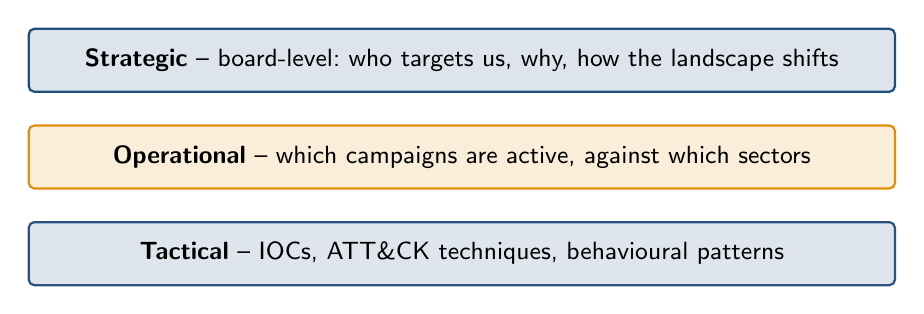
\begin{tikzpicture}[node distance=4mm]
  \node[isbox, fill=isOT!15, draw=isOT, minimum width=110mm, font=\small] (s) {\textbf{Strategic} -- board-level: who targets us, why, how the landscape shifts};
  \node[isbox, fill=isAccent!15, draw=isAccent, minimum width=110mm, font=\small, below=of s] (o) {\textbf{Operational} -- which campaigns are active, against which sectors};
  \node[isbox, fill=isPLC!15, draw=isPLC, minimum width=110mm, font=\small, below=of o] (t) {\textbf{Tactical} -- IOCs, ATT\&CK techniques, behavioural patterns};
\end{tikzpicture}
\vspace{2mm}
\begin{notebox}{All three matter}
A SOC that only consumes IOCs misses why the adversary is here in the first place. A board that only reads strategic reports misses the live campaigns this week.
\end{notebox}
\source{Bianco, D., \emph{The Pyramid of Pain}, 2013 \textbar{} Cyber Threat Intelligence Maturity Model (Sergio Caltagirone et al.).}
\end{frame}

\begin{frame}{Strategic Threat Actors Today}
\centering
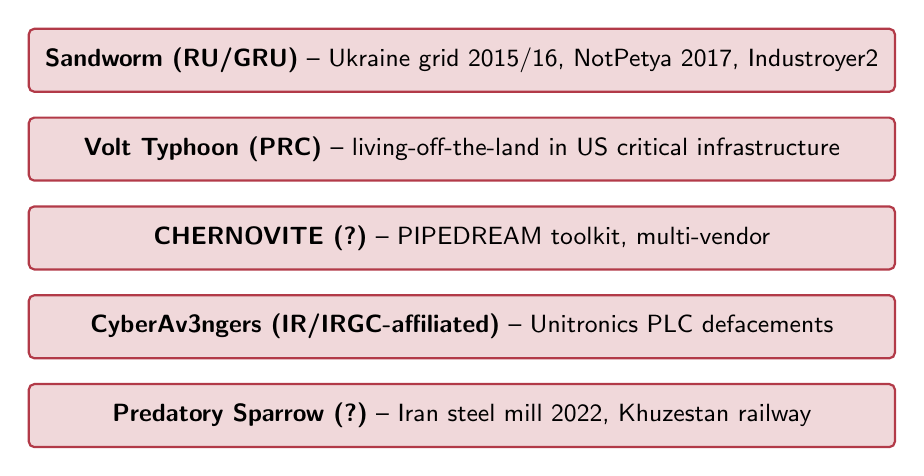
\begin{tikzpicture}[node distance=3mm]
  \node[isbox, fill=isAttack!20, draw=isAttack, minimum width=110mm, font=\small] (a) {\textbf{Sandworm (RU/GRU)} -- Ukraine grid 2015/16, NotPetya 2017, Industroyer2};
  \node[isbox, fill=isAttack!20, draw=isAttack, minimum width=110mm, font=\small, below=of a] (b) {\textbf{Volt Typhoon (PRC)} -- living-off-the-land in US critical infrastructure};
  \node[isbox, fill=isAttack!20, draw=isAttack, minimum width=110mm, font=\small, below=of b] (c) {\textbf{CHERNOVITE (?)} -- PIPEDREAM toolkit, multi-vendor};
  \node[isbox, fill=isAttack!20, draw=isAttack, minimum width=110mm, font=\small, below=of c] (d) {\textbf{CyberAv3ngers (IR/IRGC-affiliated)} -- Unitronics PLC defacements};
  \node[isbox, fill=isAttack!20, draw=isAttack, minimum width=110mm, font=\small, below=of d] (e) {\textbf{Predatory Sparrow (?)} -- Iran steel mill 2022, Khuzestan railway};
\end{tikzpicture}
\source{Dragos \emph{Year in Review} reports 2020--2024 \textbar{} CISA advisories \textbar{} Mandiant M-Trends.}
\end{frame}

\section{Sources}

\begin{frame}{The Source Stack}
\centering
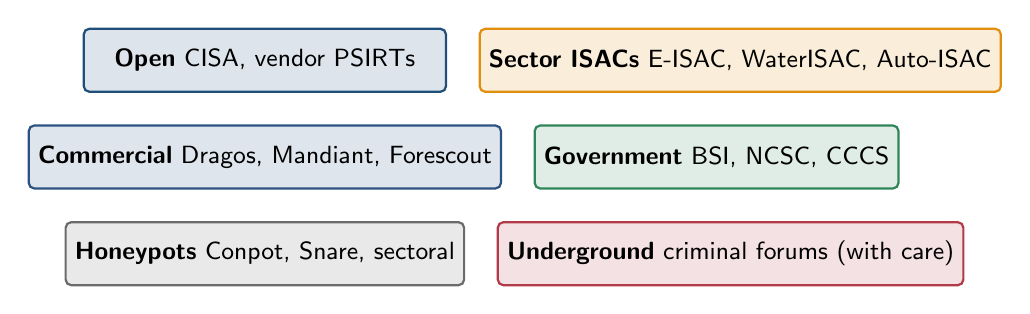
\begin{tikzpicture}[node distance=4mm]
  \node[isbox, fill=isOT!15, draw=isOT, minimum width=46mm, font=\small] (a) {\textbf{Open} CISA, vendor PSIRTs};
  \node[isbox, fill=isAccent!15, draw=isAccent, right=of a, minimum width=46mm, font=\small] (b) {\textbf{Sector ISACs} E-ISAC, WaterISAC, Auto-ISAC};
  \node[isbox, fill=isPLC!15, draw=isPLC, below=of a, minimum width=46mm, font=\small] (c) {\textbf{Commercial} Dragos, Mandiant, Forescout};
  \node[isbox, fill=isHMI!15, draw=isHMI, right=of c, minimum width=46mm, font=\small] (d) {\textbf{Government} BSI, NCSC, CCCS};
  \node[isbox, fill=isMute!15, draw=isMute, below=of c, minimum width=46mm, font=\small] (e) {\textbf{Honeypots} Conpot, Snare, sectoral};
  \node[isbox, fill=isAttack!15, draw=isAttack, right=of e, minimum width=46mm, font=\small] (f) {\textbf{Underground} criminal forums (with care)};
\end{tikzpicture}
\source{Various; quality and timeliness varies sharply -- triangulate.}
\end{frame}

\begin{frame}{Bias Awareness}
\begin{itemize}
  \item Vendor PSIRTs under-disclose -- exploits exist for years before CVE.
  \item Sector ISACs over-rotate to flagship members.
  \item Commercial intel companies push their products in the reports.
  \item Government attribution is selective and political.
  \item Underground forum chatter is partly noise and partly disinformation.
\end{itemize}
\begin{warnbox}
Treat any single source as a hypothesis. Confirm a campaign with at least two independent sources before acting on its scope.
\end{warnbox}
\source{Threat-intel methodology: Caltagirone, S. et al., \emph{Diamond Model}, 2013.}
\end{frame}

\section{Frameworks}

\begin{frame}{MITRE ATT\&CK for ICS}
\centering
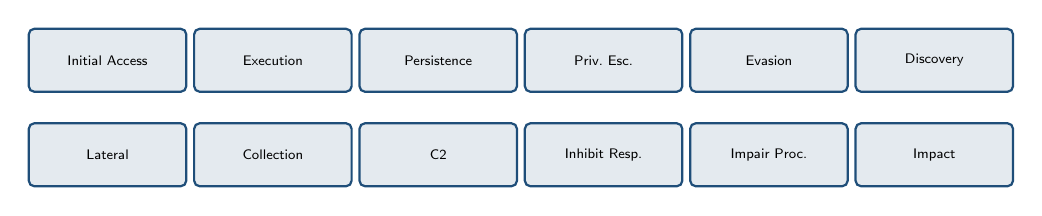
\begin{tikzpicture}[node distance=1.5mm]
  \foreach \i/\name in {0/{Initial Access},1/{Execution},2/{Persistence},3/{Priv.\ Esc.},4/{Evasion},5/{Discovery},6/{Lateral},7/{Collection},8/{C2},9/{Inhibit Resp.},10/{Impair Proc.},11/{Impact}}{
    \node[isbox, fill=isOT!12, draw=isOT, minimum width=20mm, minimum height=8mm, font=\tiny] at ({mod(\i,6)*2.1cm}, {-floor(\i/6)*1.2cm}) {\name};
  }
\end{tikzpicture}
\vspace{2mm}
\begin{notebox}{Use it for both directions}
Adversary side: which techniques did campaign X use? Defender side: what do I detect today, and where are my gaps?
\end{notebox}
\source{MITRE, \emph{ATT\&CK for ICS}, \url{https://attack.mitre.org/matrices/ics/}.}
\end{frame}

\begin{frame}{Pyramid of Pain}
\centering
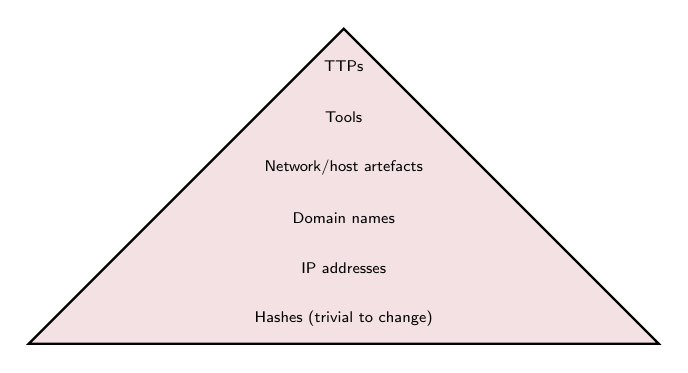
\begin{tikzpicture}[scale=0.8, transform shape]
  \draw[thick, fill=isAttack!15] (0,0) -- (10,0) -- (5,5) -- cycle;
  \node[font=\scriptsize, align=center] at (5, 0.4) {Hashes (trivial to change)};
  \node[font=\scriptsize, align=center] at (5, 1.2) {IP addresses};
  \node[font=\scriptsize, align=center] at (5, 2.0) {Domain names};
  \node[font=\scriptsize, align=center] at (5, 2.8) {Network/host artefacts};
  \node[font=\scriptsize, align=center] at (5, 3.6) {Tools};
  \node[font=\scriptsize, align=center] at (5, 4.4) {TTPs};
\end{tikzpicture}
\vspace{1mm}
\begin{notebox}{Detect higher = hurt the adversary more}
A signature on a hash dies in hours. Detection on a TTP forces the adversary to rebuild their playbook.
\end{notebox}
\source{Bianco, D., ``The Pyramid of Pain'', 2013.}
\end{frame}

\begin{frame}{Diamond Model for ICS Intrusions}
\centering
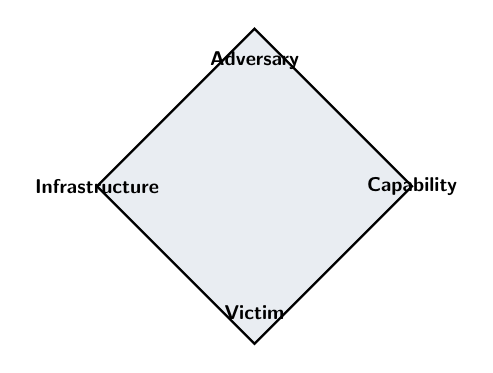
\begin{tikzpicture}[scale=0.8, transform shape]
  \draw[thick, fill=isOT!10] (0,2.5) -- (2.5,5) -- (5,2.5) -- (2.5,0) -- cycle;
  \node[font=\small\bfseries] at (2.5, 4.5) {Adversary};
  \node[font=\small\bfseries] at (5.0, 2.5) {Capability};
  \node[font=\small\bfseries] at (2.5, 0.5) {Victim};
  \node[font=\small\bfseries] at (0.0, 2.5) {Infrastructure};
\end{tikzpicture}
\vspace{1mm}
\begin{notebox}{Asking the right four questions}
Who, what, on what, against whom. Filling all four corners gives you a hypothesis that survives the next data point.
\end{notebox}
\source{Caltagirone, S., Pendergast, A., Betz, C., \emph{The Diamond Model of Intrusion Analysis}, 2013.}
\end{frame}

\section{Operational Use}

\begin{frame}{Intel-Driven Hunt}
\centering
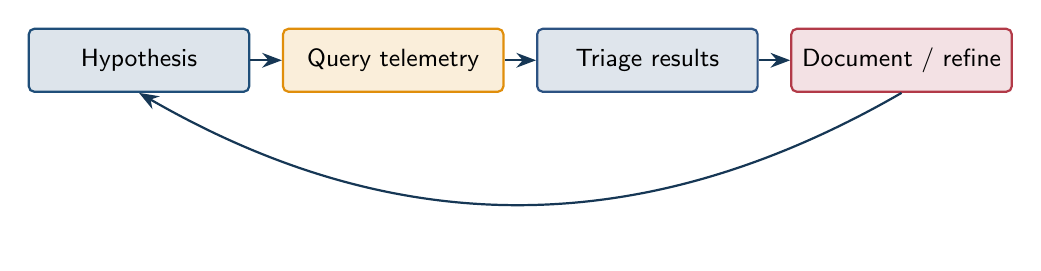
\begin{tikzpicture}[node distance=4mm]
  \node[isbox, fill=isOT!15, draw=isOT, minimum width=28mm, font=\small] (a) {Hypothesis};
  \node[isbox, fill=isAccent!15, draw=isAccent, right=of a, minimum width=28mm, font=\small] (b) {Query telemetry};
  \node[isbox, fill=isPLC!15, draw=isPLC, right=of b, minimum width=28mm, font=\small] (c) {Triage results};
  \node[isbox, fill=isAttack!15, draw=isAttack, right=of c, minimum width=28mm, font=\small] (d) {Document / refine};
  \foreach \s/\e in {a/b, b/c, c/d}{\draw[flow] (\s) -- (\e);}
  \draw[flow] (d.south) to[bend left=30] (a.south);
\end{tikzpicture}
\vspace{2mm}
\begin{notebox}{Example hypothesis}
``Volt Typhoon uses living-off-the-land via wmic and netsh. Do we see scripted wmic from non-admin hosts in the last 30 days?''
\end{notebox}
\source{SANS \emph{Threat Hunting Maturity Model}; Sqrrl/Splunk hunting playbooks.}
\end{frame}

\begin{frame}{IOC Lifecycle}
\centering
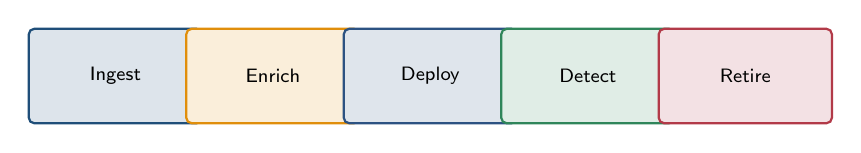
\begin{tikzpicture}[x=2cm]
  \node[isbox, fill=isOT!15, draw=isOT, font=\scriptsize, minimum width=22mm, minimum height=12mm, align=center] at (0,0) {Ingest};
  \node[isbox, fill=isAccent!15, draw=isAccent, font=\scriptsize, minimum width=22mm, minimum height=12mm, align=center] at (1,0) {Enrich};
  \node[isbox, fill=isPLC!15, draw=isPLC, font=\scriptsize, minimum width=22mm, minimum height=12mm, align=center] at (2,0) {Deploy};
  \node[isbox, fill=isHMI!15, draw=isHMI, font=\scriptsize, minimum width=22mm, minimum height=12mm, align=center] at (3,0) {Detect};
  \node[isbox, fill=isAttack!15, draw=isAttack, font=\scriptsize, minimum width=22mm, minimum height=12mm, align=center] at (4,0) {Retire};
\end{tikzpicture}
\vspace{2mm}
\begin{tipbox}{Half-life}
Network-side IOCs (IP, domain) decay in days. Host-side IOCs (file hash) decay in weeks. Behavioural rules persist for years.
\end{tipbox}
\end{frame}

\begin{frame}{STIX / TAXII -- Sharing Format}
\begin{itemize}
  \item \textbf{STIX 2.1}: structured representation of threat intel.
  \item \textbf{TAXII 2.1}: transport API for sharing STIX over HTTPS.
  \item Wide vendor support; many ISACs deliver this way.
  \item Caveat: huge volume of low-signal indicators; filter aggressively.
\end{itemize}
\source{OASIS \emph{STIX 2.1} and \emph{TAXII 2.1} specifications, 2021.}
\end{frame}

\section{Programme Building}

\begin{frame}{What an OT TI Programme Looks Like}
\centering
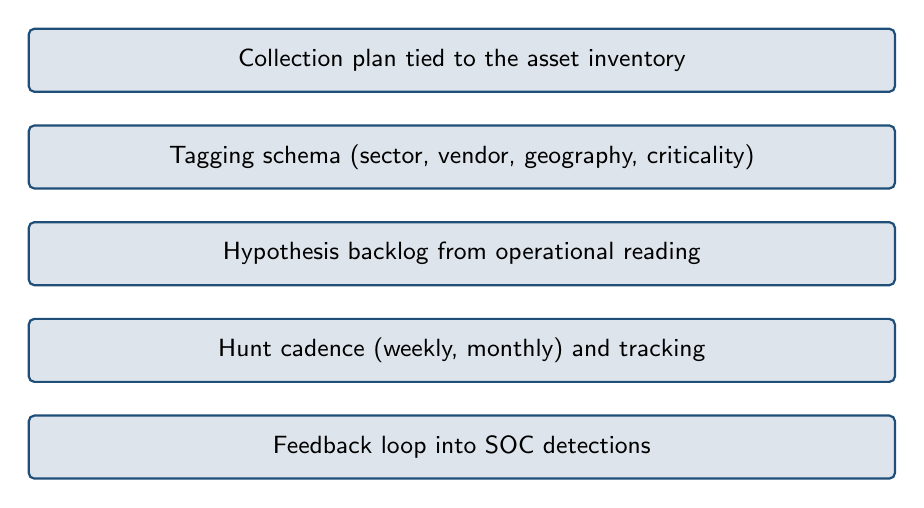
\begin{tikzpicture}[node distance=4mm]
  \node[isbox, fill=isOT!15, draw=isOT, minimum width=110mm, font=\small] (a) {Collection plan tied to the asset inventory};
  \node[isbox, fill=isOT!15, draw=isOT, minimum width=110mm, font=\small, below=of a] (b) {Tagging schema (sector, vendor, geography, criticality)};
  \node[isbox, fill=isOT!15, draw=isOT, minimum width=110mm, font=\small, below=of b] (c) {Hypothesis backlog from operational reading};
  \node[isbox, fill=isOT!15, draw=isOT, minimum width=110mm, font=\small, below=of c] (d) {Hunt cadence (weekly, monthly) and tracking};
  \node[isbox, fill=isOT!15, draw=isOT, minimum width=110mm, font=\small, below=of d] (e) {Feedback loop into SOC detections};
\end{tikzpicture}
\end{frame}

\begin{frame}{Common Failure Modes}
\begin{itemize}
  \item ``Intel'' that nobody reads (no consumer, no follow-up).
  \item IOCs deployed without context, generating alert fatigue.
  \item Detection improvements that never make it back to the platform.
  \item Single-source dependence (one vendor feed).
  \item Confusing CTI with marketing reports.
\end{itemize}
\begin{warnbox}
A CTI team without a tight feedback loop into detection engineering is decoration. Measure the time from \emph{intel published} to \emph{rule deployed}.
\end{warnbox}
\end{frame}

\begin{frame}{Sharing Responsibilities}
\centering
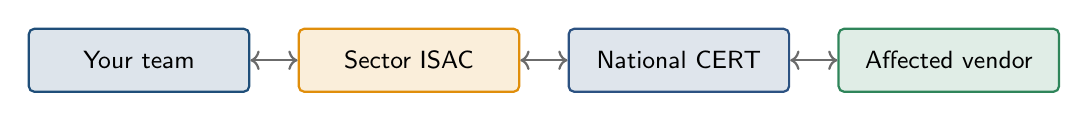
\begin{tikzpicture}[node distance=6mm]
  \node[isbox, fill=isOT!15, draw=isOT, minimum width=28mm, font=\small] (you) {Your team};
  \node[isbox, fill=isAccent!15, draw=isAccent, right=of you, minimum width=28mm, font=\small] (isac) {Sector ISAC};
  \node[isbox, fill=isPLC!15, draw=isPLC, right=of isac, minimum width=28mm, font=\small] (cert) {National CERT};
  \node[isbox, fill=isHMI!15, draw=isHMI, right=of cert, minimum width=28mm, font=\small] (vend) {Affected vendor};
  \draw[<->, thick, isMute] (you) -- (isac);
  \draw[<->, thick, isMute] (isac) -- (cert);
  \draw[<->, thick, isMute] (cert) -- (vend);
\end{tikzpicture}
\vspace{2mm}
\begin{notebox}{Reciprocity}
You get what you give. ISACs work because members share, even when it is uncomfortable. Have an internal pre-approval list of what you can share without delay.
\end{notebox}
\end{frame}

\begin{frame}{Summary -- Section \sectionNumber}
\begin{takeawaybox}{OT threat intelligence}
\begin{itemize}\setlength{\itemsep}{2pt}
  \item Three layers (strategic, operational, tactical) -- a programme delivers all three.
  \item Six source families with known biases -- triangulate, do not trust one.
  \item ATT\&CK for ICS, Diamond Model, Pyramid of Pain are the operating frameworks.
  \item Hunt with hypotheses, not haystacks; feed results back to the SOC.
  \item Measure time from intel publication to deployed detection.
\end{itemize}
\end{takeawaybox}
\end{frame}

\referencesframe{
  \item Caltagirone, S., Pendergast, A., Betz, C. \emph{The Diamond Model of Intrusion Analysis}, 2013.
  \item Bianco, D. ``The Pyramid of Pain'' blog post and presentations, 2013--2014.
  \item MITRE. \emph{ATT\&CK for ICS}, \url{https://attack.mitre.org/matrices/ics/}.
  \item Dragos. \emph{Year in Review} reports 2020--2024.
  \item Mandiant. \emph{M-Trends} annual reports.
  \item Microsoft Threat Intelligence. Volt Typhoon and related write-ups, 2023.
  \item CISA. ICS Advisories, BAS templates and IR resources.
  \item E-ISAC, WaterISAC, Auto-ISAC. Sector ISAC public summaries.
  \item BSI. \emph{Lagebericht der IT-Sicherheit in Deutschland}, annual.
  \item NCSC-UK. ICS guidance and threat reports.
  \item OASIS. \emph{STIX 2.1} and \emph{TAXII 2.1} specifications, 2021.
  \item SANS Institute. \emph{Threat Hunting Maturity Model} and related curriculum.
}

\closingframe

\end{document}
